\section{ZFOURGE SED Modelling and Model Fitting}
\subsection{Fitting ZFOURGE Photometry to SEDs}
Following the construction of theoretical AGN+Galaxy composite SED models utilising SWIRE and GALSEDATLAS galaxy templates and the SKIRTOR AGN models and the subsequent observation of colour space contamination attributable to AGN presence, we further investigated this phenomenon. This investigation employed ZFOURGE observational data and SED fitting/modelling tools. In Section 5.2, we extend our methodology to observational data, leveraging the techniques developed during the theoretical modelling phase. Specifically, we aimed to combine the ZFOURGE survey's galaxy templates with the SKIRTOR AGN models. This approach enabled us to assess the impact of AGN contamination on colour space within a real-world observational context. Given our reliance on the photometric data through the choice of the ZFOURGE survey and its auxiliary datasets, which inherently provide limited spectral information, the use of SED fitting techniques becomes essential.  Photometric observations offer only a selected sampling of a galaxy's entire SED through limited photometric bands, thus preventing the direct application of our methodology outlined in Section 5.1. To overcome this limitation, we employ SED fitting procedures to reconstruct a model of the SED based on these limited photometric data points. These models incorporate various physical processes, such as stellar evolution, dust attenuation, and emission from different stellar populations, to best fit the observed photometric data. By doing so, we generate a continuous spectrum that best characterises a galaxy's inherent bolometric flux.\\\\
We used a two-step approach to dealing with observational data, first using EAZY for direct SED fitting of photometric data. Secondly, we use CIGALE, which also allows for SED fitting and decomposes the fitted SED into its physical components. The ZFOURGE data used in this thesis contained only a subset of the full ZFOURGE observations. Data was selected based on the \texttt{use=1} where \texttt{use} flag values of 1 ensure that the source has good photometry, a reliable redshift, excellent signal-to-noise ratio and that the source hasn't been misidentified as a star. For complete information on the \texttt{use} flag, refer to Table 5 in \citet{straatman_fourstar_2016}. \\\\ We employed EAZY \citep{brammer_eazy_2008} to conduct SED fitting and generate a set of rest-frame SEDs for galaxies within the ZFOURGE survey. EAZY compares the observed multi-wavelength photometric data to a library of template SEDs, identifying the best-fitting template for each galaxy through chi-squared minimisation.  The corresponding photometric redshift derived from this process was then used to construct the rest-frame SED, enabling further analysis of the galaxy's properties
%% Explain in greater detail EAZY template extraction - using Eazy to create templates
These empirical templates were initially created for the CDFS field, with the COSMOS and UDS fields added later. The resulting SED data contained observed flux and wavelength data. The available photometric redshift from the ZFOURGE dataset was then used to convert these SEDs to the rest frame for each source. Before investigating the effect of AGN on the colour spaces of the empirical ZFOURGE template sets, we constructed a UVJ diagram using ZFOURGE photometry. This involved sampling the rest-framed ZFOURGE SEDs to create UVJ colours. The process used to sample these SEDs was the same process that was used for the theoretical template sets and involved using astSED to sample the SED in the U, V and J filters. After generating the U, V, and J colours, the same process was used to create a UVJ diagram. The recalculated UVJ colours were then plotted on the diagram and inspected to see if the recalculated UVJ diagram was qualitatively similar to the UVJ diagram created with publically available ZFOURGE photometry (See Figure \ref{fig:ZFOURGE_UVJ})
\begin{figure}[h!]
    \centering
    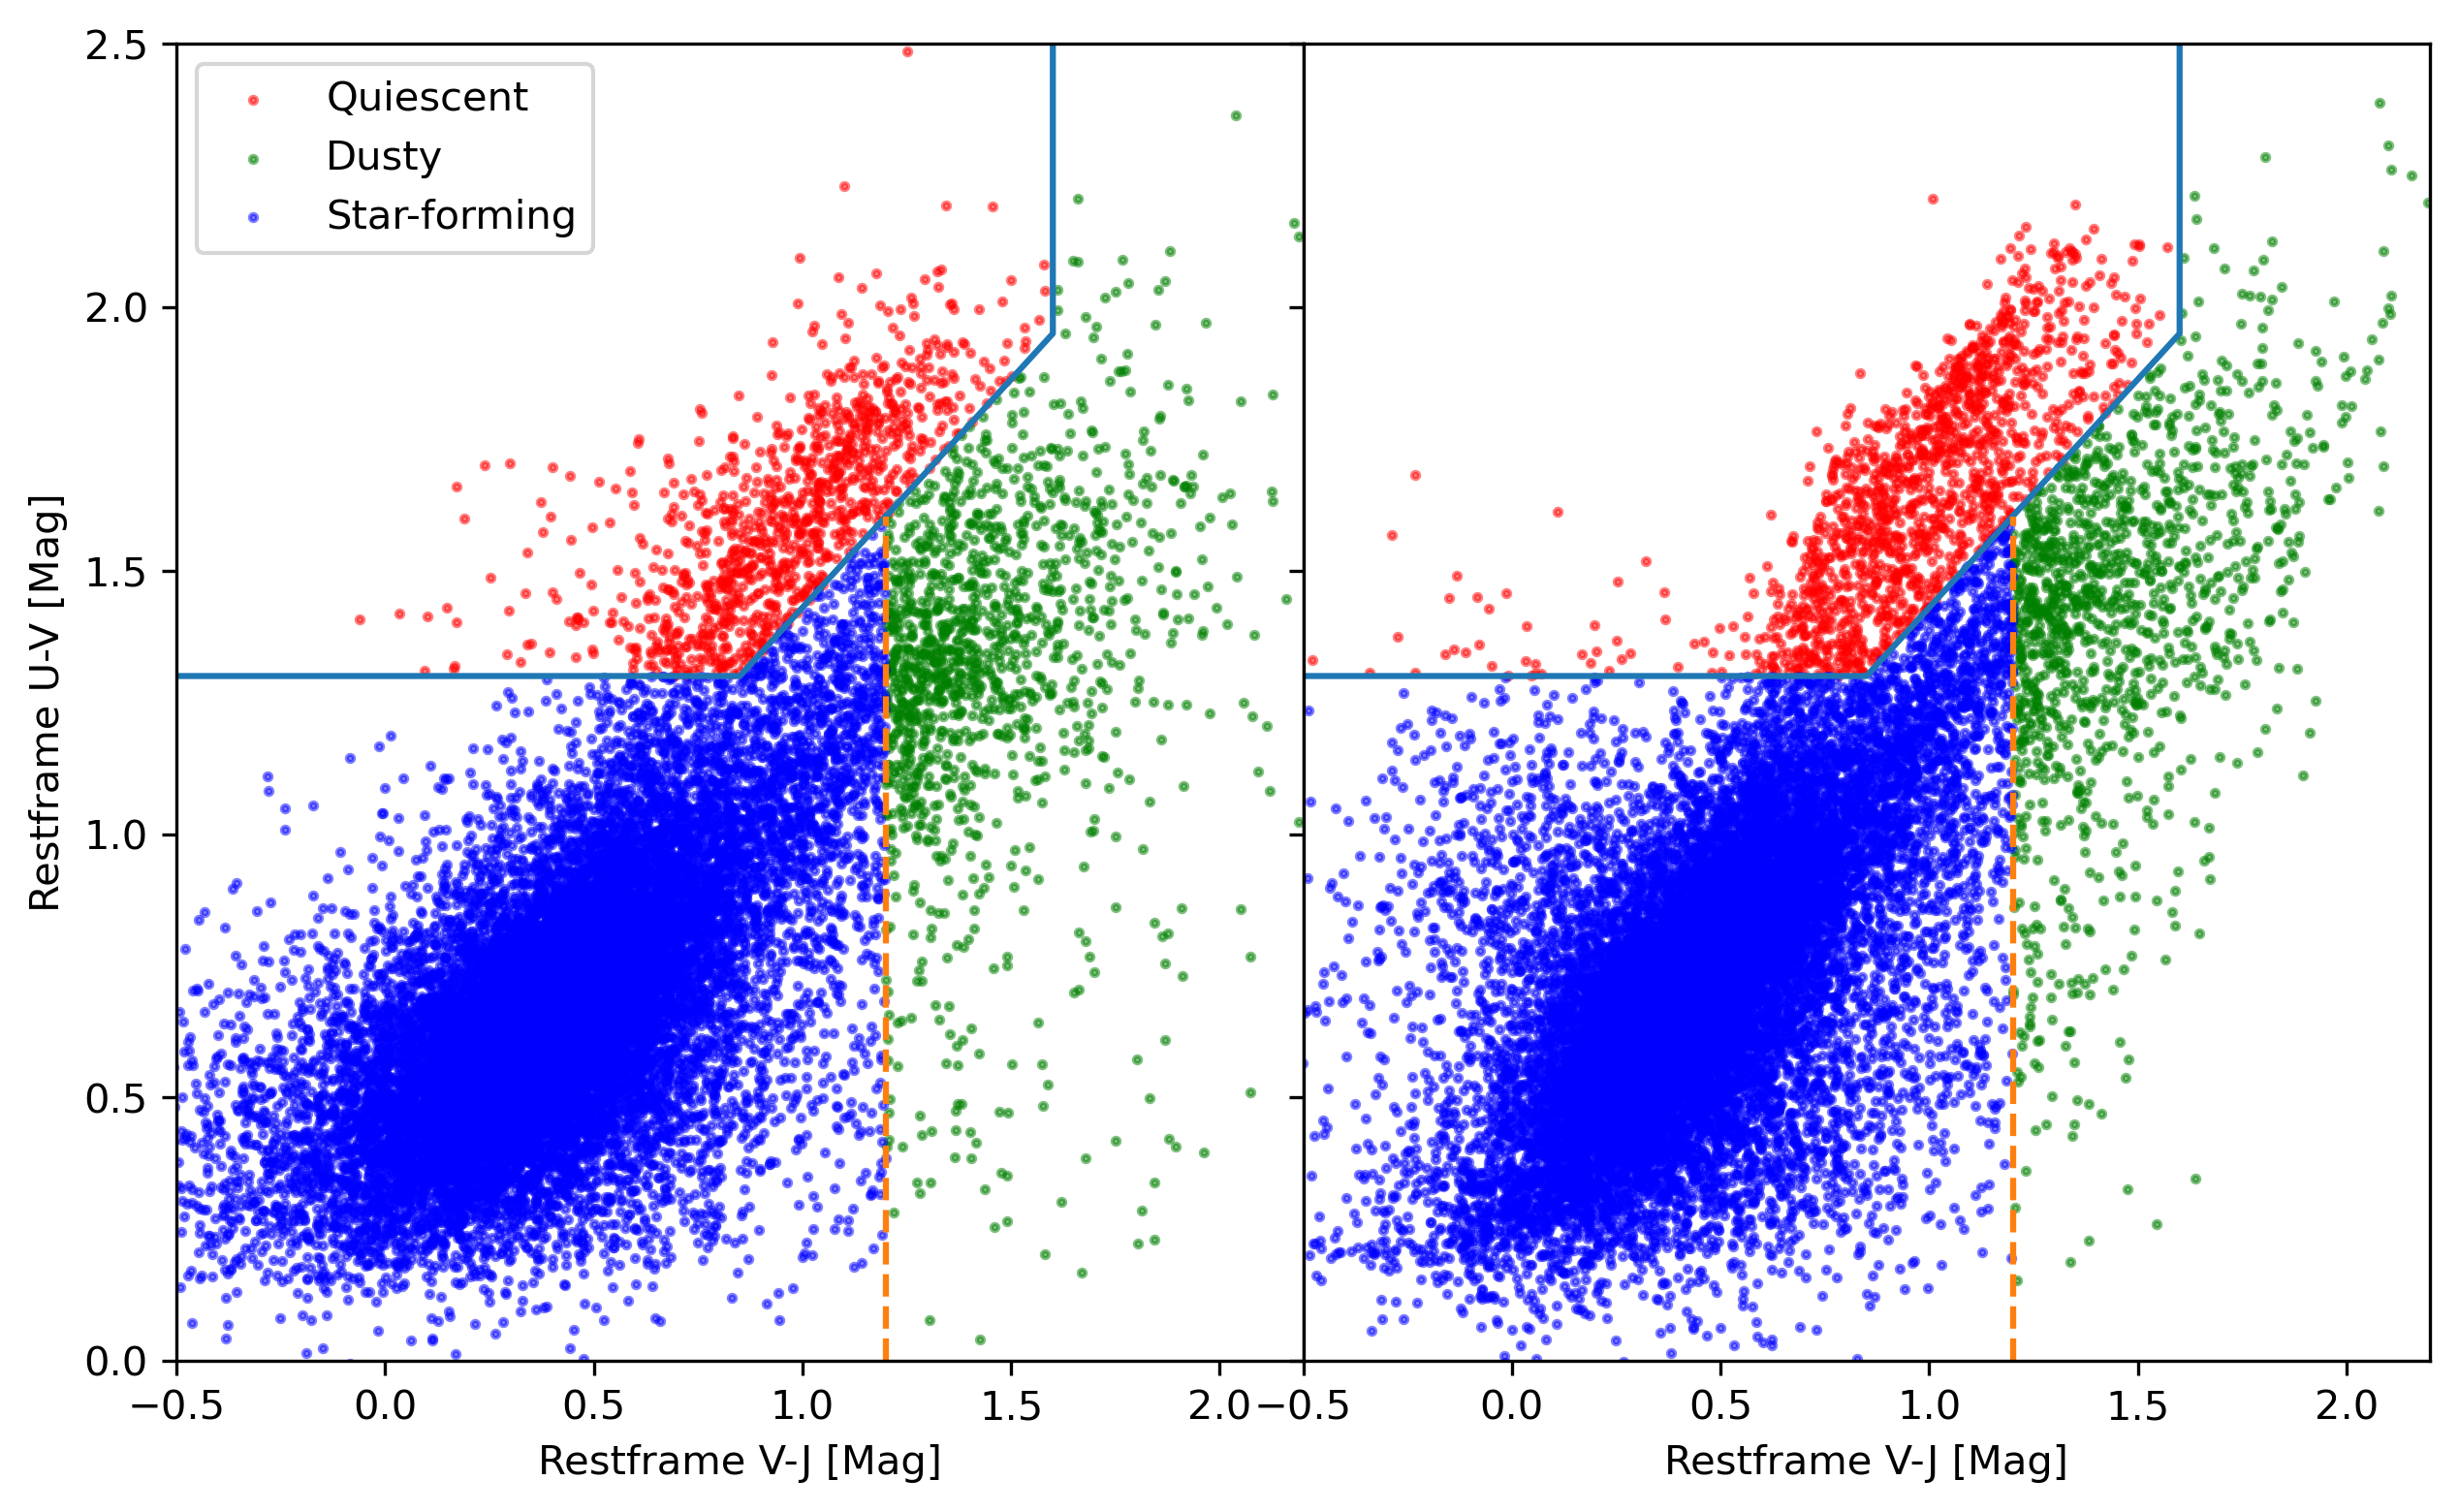
\includegraphics[width=1\linewidth]{Images/uvj_subplots.png}
    \caption{A UVJ Diagram of all fields in ZFOURGE using the original photometric data (left) and the recalculated SEDs photometrically sampled with astLib (right). Similar clustering occurs when compared with the original photometry from ZFOURGE.}
    \label{fig:ZFOURGE_UVJ}
\end{figure}\\\\
\subsection{Comparing Real and Recalculated Colours}
To ensure consistency between the original colours in ZFOURGE and the recalculated colours generated using \texttt{astSED}, we needed to check for any significant shifts in the colour space introduced by the fitting and sampling process outlined above. To check this, we calculated the vector position difference between each point.
\begin{align*}
\mathbf{v}_{\text{original}} &= \sqrt{UV^2 + VJ^2} \\
\mathbf{v}_{\text{recalculated}} &= \sqrt{UV_0^2 + VJ_0^2} \\
\|\Delta \mathbf{v}\| &= \|\mathbf{v}_{\text{original}} - \mathbf{v}_{\text{recalculated}}\|
\end{align*}
We calculated the vector offset for each galaxy in the UVJ diagram using this equation. To assess the magnitude of these offsets, we generated a distribution of their absolute values. This allowed us to check for any significant shifts in the colour space introduced by our recalculation process. (See Figure \ref{fig:vector_mag_difference})

Using this method, we confirmed that our calculation method caused only a minor difference in UVJ positions. Thus, creating composites using the ZFOURGE SEDs with the AGN models was possible. A set of composite SEDs was constructed from the ZFOURGE survey data, following the methodology described in Section 5.1.3. This process yielded approximately 200,000 composite SEDs, spanning a range of AGN contribution values. Each SED was then sampled using the \texttt{astLib} library to determine the corresponding UVJ and ugr colours across the different AGN contribution levels. To assess the impact of incorporating ZFOURGE data into the composite modelling, a series of colour-colour diagrams was generated, one for each AGN contribution value. These diagrams were compared against those derived from purely theoretical models to evaluate the consistency between the two approaches. A subset of these composite SEDs was selected based on minimal shifts in their colour-space positions. The IDs and redshifts of these selected SEDs were then used to construct a subsample for bootstrapping. This bootstrapping process ensured a redshift distribution consistent with that of the parent ZFOURGE survey. Finally, the IDs of the bootstrapped subsample were exported and used to retrieve the corresponding decomposed SEDs from the CIGALE dataset.
\begin{figure}[h!]
    \centering
    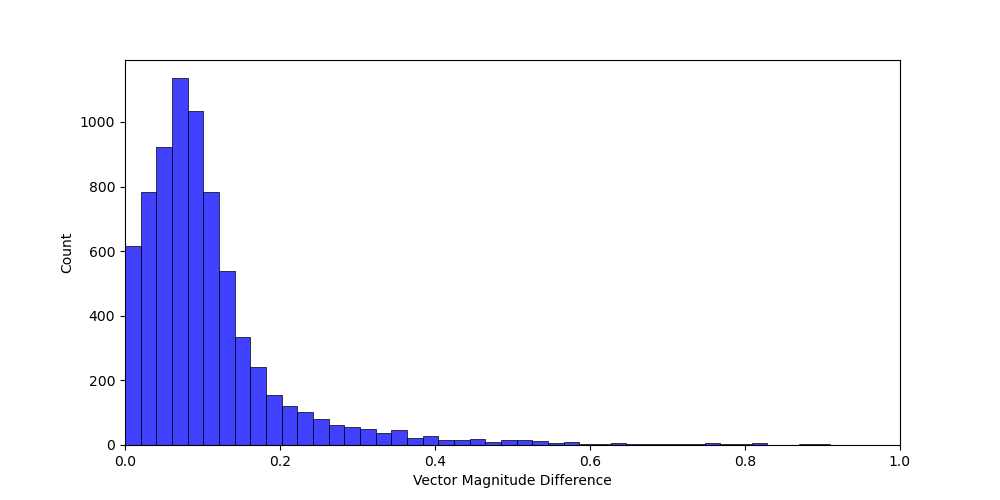
\includegraphics[width=1\linewidth]{Images/vector_magnitude_difference_cdfs_example.png}
    \caption{Distribution of vector magnitude differences from a sample of sources from ZFOURGE, showing how UVJ positions changed by recalculating them with the astLib and from ZFOURGE SEDs fit using EAZY.}
    \label{fig:vector_mag_difference}
\end{figure}
\subsection{Decomposed SEDs using CIGALE}
To examine how much each source's light comes from an AGN, we need to separate the AGN's contribution from the rest of the galaxy's light within the SED. We used CIGALE (Code for Investigating Galaxy Emission; \citealt{burgarella_star_2005}; \citealt{noll_analysis_2009}; \citealt{boquien_cigale_2019}), a SED fitting tool, to analyse the ZFOURGE photometry using a Bayesian approach.  Once the best-fit SED was determined, a decomposition technique was used to isolate the light from different physical processes within the galaxy. A description of how this decomposition process was carried out can be found in Section 3.3 of \citet{cowley_decoupled_2018}. The result of this spectral decomposition process was a model spectrum that completely isolated the AGN flux by systematically separating contributions from various astrophysical components, including stellar populations (both young and old), nebular emission and absorption features, dust, the galactic continuum, attenuated light, and the intergalactic medium. The result was a SED containing many best-fit components of a composite source (See Figure \ref{fig:decomposed_sed_6455}). 
\begin{figure}[h!] % May replace this different decomposed SED if appropriate
    \centering
    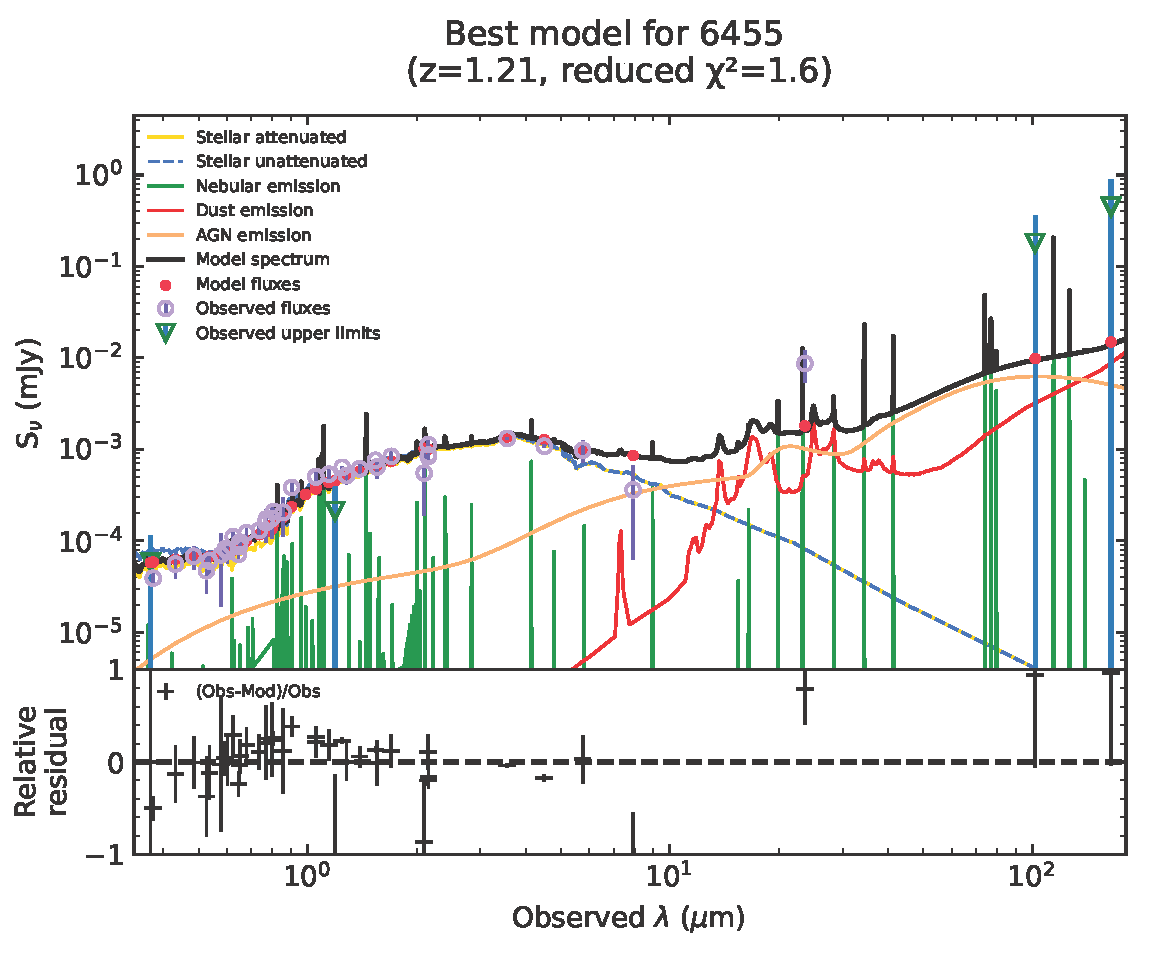
\includegraphics[width=0.6\linewidth]{Images/6455_best_model.png}
    \caption{Galaxy CDFS6455 from the ZFOURGE Survey that has been decomposed into constituent components using CIGALE}
    \label{fig:decomposed_sed_6455}
\end{figure} \\\\
 Following the decomposition process, the source's AGN component was completely isolated and kept aside. This allowed for two basic SEDs to be investigated: a complete SED containing all physical components and a decomposed SED with the AGN component completely removed. The complete SED and the AGN-removed SED were then sampled using astLib to create UVJ and ugr colours using the methodology outlined in 5.1.4. This allowed for a selection of UVJ and ugr positions to be calculated and compared with the associated positions obtained from the ZFOURGE catalogue; utilising the vector displacement equation, it was possible to inspect if there was a statistically significant change in positions due to the decomposition technique. After determining that the position change would not affect the analysis, the UVJ and ugr positions of the AGN-removed SEDs were calculated. By comparing the positions of the complete and AGN-removed SEDs, we assessed the impact of the AGN on the ZFOURGE galaxy colours. 
